123123123
\subsection{Introduction}
456456456
As computing paradigms are shifting to cloud-centric technologies, users
of these technologies are increasingly concerned with the privacy and
confidentiality of the data they upload to the cloud. Specifically, a
\emph{client} uploads data to the \emph{server} and expects the
following guarantees: 

\BEN
\item The uploaded data should remain private, even
from the server itself;
\item The server should be able to perform computations on the uploaded
data in response to client queries;
\item The client should be able to efficiently recover the results of
the server's computation with minimal post-processing.
\EEN

In this work, we will focus on the computational task of secure search.
In this application, the client uploads a set of records to the server,
and later posts queries to the server.  Computation proceeds in two
steps called \emph{matching} and \emph{fetching}.
%
In the matching step, the server compares the encrypted search query from
the client with all encrypted records in the database, and computes an
encrypted 0/1 vector, with 1 indicating that the corresponding record
satisfies the query.  The fetching step returns all the 1-valued
indexes and the corresponding records, to the client for decryption.

While seemingly conflicting goals, the guarantees of (1), (2), (3) can
be simultaneously achieved for the secure search setting via techniques
such as secure multiparty computation and searchable encryption.
Recently, a line of works has focused on Fully Homomorphic Encryption
(FHE)-based secure search, which we describe next.


\paragraph{FHE-based secure search.}
The simplicity of the framework of {\em secure search on FHE encrypted
data} is attractive. Compared to other secure search systems, no costly
setup procedure is necessary; it is sufficient for the client merely to
upload the encrypted database to the server. Confidentiality is provided
because the server works only on the encrypted query and records. The
server can still perform the search correctly due to the powerful
property of the full homomorphism of the underlying encryption scheme. 

For this reason, researchers have been paying increasing attention to
this problem. In particular, Akavia et~al.~\cite{CCS:AkaFelSha18}
introduce a framework of performing secure search on FHE-encrypted data
(see Figure~\ref{fig:secure-search}). 

\begin{figure}
\centering
\includegraphics[width=3.5in]{src/securesearch/pic.pdf}
%\centering
%\includegraphics[width=6in]{pic.pdf}

% \hspace{\footnotesize In the above, $\lbra \cdot \lket$ denotes
% an FHE-encrypted ciphertext.}

\hspace{-4em}{\footnotesize In the above, $\lbra \cdot \lket$ denotes
an FHE-encrypted ciphertext.}

\caption{The secure search framework in~\cite{CCS:AkaFelSha18}}
\label{fig:secure-search}
\end{figure}

Informally, a secure, homomorphic encrypted search scheme has the
following Setup: 
\BEN
\item (Setup) The client encrypts and uploads $n$ items $x = (x_1, \ldots, x_n)$
to the server. Let $\lbra x \lket = (\lbra x_1
\lket, \ldots, \lbra x_n \lket).$ denote the encrypted data stored in
the server. 
\EEN

Throughout the paper, we let $\lbra \cdot \lket$ denote an FHE-encrypted
ciphertext. After the encrypted records have been uploaded, the client
can perform a secure search using three algorithms, (Query, Match,
Fetch).
\BEN
\setcounter{enumi}{1}
\item (Query) The client sends an encrypted query $\lbra q \lket$ to the server.  

\item (Match) The server homomorphically evaluates the query $\lbra q \lket$ on
each record $\lbra x_i \lket$ to obtain the encrypted matching
results $\lbra b \lket = (\lbra b_1 \lket, \ldots, \lbra b_n \lket).$
That is, $b_i$ is 1 if item $x_i$ satisfies the given query $q$;
otherwise, $b_i$ is $0$.

\item (Fetch) Given $\lbra b \lket$, the server homomorphically computes
$\lbra i^* \lket$, where $i^* = \min \{ i \in [n] : b_i = 1 \}$ which
corresponds to the first matching record index. It fetches  $\lbra
x_{i^*} \lket$ (obliviously) and sends $(\lbra i^* \lket, \lbra x_{i^*}
\lket)$ to the client for decryption. 
\EEN

\paragraph{Multiplications in the fetching step.}
Akavia et al.~also provide a construction that performs the fetching
step in $O(n \log^2 n)$ homomorphic multiplications. Subsequently, more
efficient algorithms have been presented with $O(n \log n)$
multiplications~\cite{PETS:AGHL19} and $O(n)$
multiplications~\cite{CCS:WYXZ20}.

\subsubsection{Motivation}
\paragraph{Bottleneck: fetching records sequentially.}
Suppose a client wants to fetch all matching items.  Under the above
framework, the client would first obtain the first matching index $i^*$
and its corresponding item $x_{i^*}$.  To fetch the second matching
item, the framework suggests that the client should slightly change the
original query $q$ to a new query $q'_{i^*}$ as follows:

\BI
\item $q'_{i^*}(i, x_i)$ return true if $q(i, x_i)$ is true and $i > i^*$. 
\EI

Then, by executing a new instance of the protocol with the encrypted
query $\lbra q'_{i^*} \lket$, the client will obtain the second matching
item.  By repeating this procedure, the client will ultimately obtain
all the matching records.  

Note that the query $q'_{i^*}$ embeds $i^*$ in itself as a constant,
which implies that there is no way for the client to construct this
query $q'_{i^*}$ without obtaining $i^*$ first. In other words, the
client can construct the query for the second matching item, {\em only
after fetching the first matching item}. In this sense, the framework
inherently limits the client to fetch only a single matching record at a
time in a sequential manner. 

If there are $\ell$ matching records, the client and server have to
execute $\ell$ instances of the Query, Match, and Fetch algorithms.
Since each Match and Search step requires costly homomorphic
multiplications, the limitation of sequential protocol execution creates
a serious bottleneck with respect to the running time. This leads us to
ask the following natural question:

\medskip

\BI
\item[]
\it
Is there a different secure search framework that allows the client to
fetch all the matching records by executing a smaller number of protocol
executions, possibly avoiding sequential record fetching?
\EI

\paragraph{Reducing homomorphic multiplications.} 
All previous schemes have to perform $\Omega(n)$ homomorphic
multiplications in the fetching step. Since homomorphic multiplications
are costly operations, it is desirable to reduce such computations,
which begs the natural following question: 

\medskip
\BI
\item[]
\it
Can you reduce the number of homomorphic multiplications in the fetching
step? 
\EI
In this paper, we answer both of the above questions affirmatively. 

\begin{figure*}
\begin{tabular}{lccccccc}
%\begin{tabular*}{\textwidth}{c @{\extracolsep{\fill}} lccccccc}
%\small
\hline 
  & rounds & \#Match & ${\sf hmult}$ & ${\sf hadd}$ & ${\sf smult}$ & communication  & plaintext modulus \\
\hline 
LEAF~\cite{CCS:WYXZ20}    & $s$ & $s$ & $O(ns)$   &  $O(ns\log n)$     & 0      & $O(s \cdot \log n \cdot |C|)$ & 2 \\ 
Protocol w/ BF-COIE   & $3$ & 1 &  0 & $O(n \log \frac n s)$ & 0               & $O(s^{1+\e} \log \frac n s \cdot |C| + pir(s))$ & prime \\
Protocol w/ PS-COIE   & $3$ & 1 & 0 & $n \cdot s$   &  $n \cdot s$                  & $O(s \cdot |C| + pir(s) )$ & prime \\ 
Protocol w/ BFS-CODE  & $2$ & 1 & $n$    &    $O(\secparam n)$ &   0        & $O(s \secparam \cdot |C|)$ & prime \\ 
\hline
\end{tabular}


\BI
\item $\secparam$: statistical security parameter.
\item $n$: number of uploaded encrypted records.
\item $s$: number of matching records. 
\item $\e$: protocol parameter such that $0 < \e < 1$.
\item \#Match: number of times the matching algorithm is executed. 
\item ${\sf hmult}$: number of homomorphic multiplication operations
used in the overall fetching step.
\item ${\sf hadd}$: number of homomorphic addition operations used in the overall fetching step. 
\item ${\sf smult}$: number of scalar (plain) multiplication
operations used in the overall fetching step.
\item $|C|$: length of an FHE ciphertext.
\item $pir(s)$: communication complexity required to retrieve $s$ records via a PIR protocol. 
\EI

\caption{Performance Comparisons when $s$ records are fetched\label{fig:comparison}}
\end{figure*}


\subsubsection{Our Work}
\paragraph{Parallelizing the Fetch procedure.}
To address the issues, we introduce a new secure search framework where
the matching items are retrieved {\em in parallel} in a constant number
of rounds.  Our Setup, Query and Match algorithms are the same as in
prior work.  However, we modify the Fetch 
procedure, dividing into two steps:~Encode
and Decode.  In the Encode step, the server 
homomorphically inserts the matching items 
into a data structure - the particular structure depends on the construction, as
we provide 3 different constructions, each using a different encoding.  
%
After receiving the encrypted encoding, the 
client decrypts the encoding and runs the Decode step to recover the items.  

\paragraph{Compressed oblivious encoding.}
The encoding is computed homomorphically, and, most importantly, allows
to encode {\em the full result set}, rather than just a single item.  
In particular, we introduce a notion of Compressed Oblivious Encoding (COE).  A compressed oblivious encoding takes as input a large, but sparse, vector and compresses it to a much smaller encoding from which the non-zero entries of the original vector can be recovered.  What makes this encoding \emph{oblivious} is that the encoding procedure is performed on encrypted data.  
In certain constructions, the encoding includes the data values (CODE, compressed oblivious data encoding), and in
others it only includes the indices (COIE, compressed oblivious index encoding).  In the latter case, the Decode
procedure is interactive, and allows the client to recover the values
from the decoded set of indices.  

For simplicity, when describing the 
generic syntax of secure search scheme, we denote the Encode procedure as taking both the
indices and the values as input, and we suppress the fact that when the
values are not used during Encoding, the Decoding step must be
interactive. Recall, we use $\lbra b \lket = (\lbra b_1\lket, \ldots, \lbra b_n \lket)$
to denote the encrypted bit vector that results from the Match step. 

\BEN
\setcounter{enumi}{3}
\item (Encode) Let $S = \{ i \in [n] : b_i = 1 \}$.  Let $V = \{v_i : i \in S\}$. The server
homomorphically evaluates an $\lbra \mathsf{encoding}(S,V) \lket$ and send it to
the client. 
\item (Decode) The client decrypts $\lbra
\mathsf{encoding}(S) \lket$ and runs the decoding 
procedure to recover $(S, V)$.
\EEN

We assume that the results set $|S|$ is small (i.e., sublinear in $n$).
%
We would like the size of the compressed encoding to be sublinear in $n$ to
maintain meaningful communication cost. 

\paragraph{No multiplications in the Encode step.} 
To ensure minimal computational cost for encoding the results, we also wish to
minimize the number of homomorphic multiplications.  Recall, the best prior
work requires $O(n)$ multiplications by the server.  Somewhat surprisingly, we
demonstrate three encoding algorithms that can be evaluated {\em without} any
homomorphic multiplications! 


\paragraph{Using PIR (Private Information Retrieval).} 
The asymptotic complexities and trade-offs of the search protocols are presented in
Figure~\ref{fig:comparison}.

In some of our
protocols (i.e., the search protocols with BF-COIE and PS-COIE; see Sections 4 and 6.3 for more detail), the indices and actual records are fetched in separate steps.  This allows us to focus on optimizing the retrieval of the indices after which the values can be fetched using an efficient (setup-free) PIR protocol resulting in overall savings.  

However, if reliance on PIR is undesirable, we also offer a variant that fetches the values directly (i.e., the protocol w/ BFS-CODE in Figure~\ref{fig:comparison}; see Sections 5 and 6.4 for more detail), as in prior work.


% Due to this approach, those protocols can benefit from employing more
% efficient setup-free PIR protocols, at the expense of increasing the
% round complexity by 1. For
% example, we can also employ a 2-server PIR scheme based on \
% functional secret sharing~\cite{CCS:BoyGilIsh16}, which is setup-free
% and very efficient.  However, we stress that if this is undesirable, \dov{is this ok?} and if the cost of single-server PIR is deemed to be too high, two \dov{?} of the Fetch protocols that we present allow for direct recovery of the values without the PIR step, as in prior work.  

\paragraph{Implementation.} We implement all of our proposed schemes and
compare their performance with that of prior work. Our experiments show
that our schemes outperform the fetching procedure of prior work by a
factor of 1800X when fetching 16 records, which results in a 26X speedup
for the full search functionality.


% our
% schemes outperforms the previous scheme by about 100-1000 times.

\iffalse
\paragraph{Our contributions.} 
We summarize our contributions as follows: 
\BI
\item {\em New framework.} We provide a new framework for secure search
based on FHE schemes that the client fetches the matching records in
parallel.

\item {\em Three schemes.} We provide three schemes that fit into our
new framework. All the schemes preform the searching step without any
expensive homomorphic multiplications. 

\item {\em Implementation.} We implement our schemes and compare the
performance of the schemes with the previous work. 
\snote{edit after the measurement} Our experiment shows
that our schemes outperforms the previous scheme by 10-100 times. 
\EI
\fi


